\documentclass[11pt, a4paper]{article}
\usepackage[utf8]{inputenc}
\usepackage[margin=1in]{geometry} %Sets proper 1-inch margins. 
\usepackage{amsmath} %Only load this if you are using math/equations.
\usepackage{graphicx} %Only need to call this if inserting images.
\usepackage{caption} %Only need to call this if inserting captions.
\usepackage{float} %Allows the use of the [H] specifier. 
\graphicspath{{C:/Users/jonah/Pictures/meme/}} %Sets the working directory for images.
\usepackage[colorlinks,citecolor=blue,linkcolor=blue,urlcolor=blue]{hyperref} %Allows for the embedding of urls. 
\usepackage{setspace}
\usepackage{blindtext}

\pagenumbering{arabic}

\usepackage{fancyhdr}

\pagestyle{fancy}
\fancyhf{}
\rhead{Jonah Edmundson \\ Jan 2023}
\lhead{\thepage}

\newcommand{\comment}[1]{}

\usepackage{Sweave}
\begin{document}
\Sconcordance{concordance:datacleaning.tex:datacleaning.Rnw:%
1 22 1 1 0 30 1 1 2 1 0 1 12 11 0 1 2 5 0 1 1 5 0 1 3 1 0 1 1 1 2 45 0 %
1 2 4 1 1 3 7 0 1 4 2 0 1 4 8 0 1 2 2 1 1 2 6 0 2 1 6 0 1 2 4 1 1 3 2 0 %
1 4 3 0 2 1 7 0 1 4 2 0 1 2 15 0 1 13 11 0 1 5 3 0 6 1 1 4 2 0 1 3 13 0 %
1 3 1 0 4 1 3 0 1 2 9 1 1 5 4 0 1 1 6 0 1 2 6 1 1 2 1 0 1 8 7 0 1 11 9 %
0 1 2 1 0 2 1 7 0 1 4 2 0 1 1 5 0 1 2 1 0 1 1 6 0 1 2 4 1 1 4 3 0 4 1 %
15 0 2 1 1 2 1 0 1 1 1 4 2 0 1 2 7 0 1 1 6 0 1 11 10 0 1 2 7 0 1 1 6 0 %
1 4 10 0 1 2 1 1 1 35 2 1 1 12 7 1 1 4 3 0 1 1 53 0 1 2 6 1 1 5 4 0 1 1 %
8 0 1 2 3 1 1 28 27 0 1 2 3 0 1 2 3 1 1 3 2 0 1 3 1 0 1 6 4 0 1 1 7 0 1 %
3 1 0 1 1 1 44 43 0 2 1 26 0 1 2 2 1 1 3 8 0 1 3 1 0 1 1 3 0 1 2 2 1 1 %
2 1 0 1 1 68 0 1 2 5 1 1 2 4 0 1 2 2 1}


\begin{center}
\Large{\textsc{Data Cleaning}}
\par
\normalsize{\textsc{for}}
\par
\large{\textsc{Kelowna Weather-Crash Project}}
\end{center}


\vspace{0.917 pc} %Creates a paragraph line break. 

\section*{Section 1}


remove all 'flag' variables

group weather data based on time groups in crash dataset, then join weather data on crash table (1 case = 1 crash, what was the weather like when this crash occurred?)

is 'weather' reliable? may need to correct it if there is precipitation but NA for 'weather'

Loading in weather data:

\begin{Schunk}
\begin{Sinput}
> fullWeather = c()
> for (i in c(2017:2021)){
+   for (j in c(1:12)){
+     temp = subset(read.csv(paste0('../../weatherdata/en_climate_hourly_BC_1123939_', 
+       sprintf("%02d", j), '-', i, '_P1H.csv')), 
+       select = - c(`Temp.Flag`, 
+       `Dew.Point.Temp.Flag`, `Rel.Hum.Flag`,
+       `Precip..Amount.Flag`, `Wind.Dir.Flag`, 
+       `Wind.Spd.Flag`, `Visibility.Flag`, 
+       `Stn.Press.Flag`, `Hmdx`, `Hmdx.Flag`, `Wind.Chill.Flag`))
+     fullWeather = rbind(fullWeather, temp)
+   }
+ }
> nrow(fullWeather)
\end{Sinput}
\begin{Soutput}
[1] 43824
\end{Soutput}
\begin{Sinput}
> 24*365*5 + 24 #2020 was a leap year
\end{Sinput}
\begin{Soutput}
[1] 43824
\end{Soutput}
\begin{Sinput}
> #assigning a Julian day variable
> library(lubridate)
> fullWeather$julianday = yday(as.Date(fullWeather$Date.Time..LST., tz='LST'))
> summary(fullWeather)
\end{Sinput}
\begin{Soutput}
 Longitude..x.     Latitude..y.    Station.Name     Climate.ID     
 Min.   :-119.4   Min.   :49.96   KELOWNA:43824   Min.   :1123939  
 1st Qu.:-119.4   1st Qu.:49.96                   1st Qu.:1123939  
 Median :-119.4   Median :49.96                   Median :1123939  
 Mean   :-119.4   Mean   :49.96                   Mean   :1123939  
 3rd Qu.:-119.4   3rd Qu.:49.96                   3rd Qu.:1123939  
 Max.   :-119.4   Max.   :49.96                   Max.   :1123939  
                                                                   
         Date.Time..LST.       Year          Month             Day       
 2017-01-01 00:00:    1   Min.   :2017   Min.   : 1.000   Min.   : 1.00  
 2017-01-01 01:00:    1   1st Qu.:2018   1st Qu.: 4.000   1st Qu.: 8.00  
 2017-01-01 02:00:    1   Median :2019   Median : 7.000   Median :16.00  
 2017-01-01 03:00:    1   Mean   :2019   Mean   : 6.524   Mean   :15.73  
 2017-01-01 04:00:    1   3rd Qu.:2020   3rd Qu.:10.000   3rd Qu.:23.00  
 2017-01-01 05:00:    1   Max.   :2021   Max.   :12.000   Max.   :31.00  
 (Other)         :43818                                                  
   Time..LST.      Temp...C.       Dew.Point.Temp...C.  Rel.Hum....    
 00:00  : 1826   Min.   :-28.900   Min.   :-32.800     Min.   : 12.00  
 01:00  : 1826   1st Qu.:  0.800   1st Qu.: -2.100     1st Qu.: 52.00  
 02:00  : 1826   Median :  7.800   Median :  2.300     Median : 74.00  
 03:00  : 1826   Mean   :  8.511   Mean   :  2.043     Mean   : 69.33  
 04:00  : 1826   3rd Qu.: 15.700   3rd Qu.:  7.500     3rd Qu.: 89.00  
 05:00  : 1826   Max.   : 43.800   Max.   : 19.700     Max.   :100.00  
 (Other):32868   NA's   :30        NA's   :29          NA's   :24      
 Precip..Amount..mm. Wind.Dir..10s.deg. Wind.Spd..km.h.  Visibility..km.
 Min.   :0.00000     Min.   : 1.00      Min.   : 0.000   Min.   : 0.0   
 1st Qu.:0.00000     1st Qu.: 9.00      1st Qu.: 4.000   1st Qu.:16.1   
 Median :0.00000     Median :18.00      Median : 5.000   Median :16.1   
 Mean   :0.02999     Mean   :19.13      Mean   : 8.415   Mean   :15.1   
 3rd Qu.:0.00000     3rd Qu.:33.00      3rd Qu.:11.000   3rd Qu.:16.1   
 Max.   :7.10000     Max.   :36.00      Max.   :58.000   Max.   :16.1   
 NA's   :24          NA's   :13955      NA's   :52       NA's   :31     
 Stn.Press..kPa.   Wind.Chill         Weather        julianday    
 Min.   :93.73   Min.   :-34.00   Rain    : 2069   Min.   :  1.0  
 1st Qu.:96.10   1st Qu.:-11.00   Snow    : 1662   1st Qu.: 92.0  
 Median :96.52   Median : -6.00   Haze    : 1187   Median :183.0  
 Mean   :96.55   Mean   : -8.22   Fog     :  873   Mean   :183.1  
 3rd Qu.:96.96   3rd Qu.: -4.00   Rain,Fog:  233   3rd Qu.:274.0  
 Max.   :99.34   Max.   : -1.00   (Other) :  246   Max.   :366.0  
 NA's   :34      NA's   :36294    NA's    :37554                  
\end{Soutput}
\end{Schunk}

\pagebreak

There are 22 empty strings in the \texttt{Weather} variable that should be NAs.

\begin{Schunk}
\begin{Sinput}
> length(fullWeather[fullWeather$Weather == "" &
+               is.na(fullWeather$Weather) == FALSE, "Weather"])
\end{Sinput}
\begin{Soutput}
[1] 22
\end{Soutput}
\begin{Sinput}
> ## SETTING EMPTY TO NA
> fullWeather$Weather[fullWeather$Weather == "" &
+               is.na(fullWeather$Weather) == FALSE] = NA
> ## CHECKING
> length(fullWeather[fullWeather$Weather == "" &
+               is.na(fullWeather$Weather) == FALSE, "Weather"])
\end{Sinput}
\begin{Soutput}
[1] 0
\end{Soutput}
\end{Schunk}

Need to relevel factor to remove empty string option:

\begin{Schunk}
\begin{Sinput}
> "" %in% levels(fullWeather$Weather)
\end{Sinput}
\begin{Soutput}
[1] TRUE
\end{Soutput}
\begin{Sinput}
> fullWeather$Weather = droplevels(fullWeather$Weather)
> "" %in% levels(fullWeather$Weather)
\end{Sinput}
\begin{Soutput}
[1] FALSE
\end{Soutput}
\end{Schunk}

\pagebreak

Changing \texttt{Weather} factor variable to many indicator variables. 

\begin{Schunk}
\begin{Sinput}
> #creating columns
> lst = c()
> for (i in levels(fullWeather$Weather)){
+   temp = unlist(strsplit(as.character(i), ","))
+   lst = c(lst, temp)
+ }
> lst = lst[!(duplicated(lst))] #removing duplicates
> lst
\end{Sinput}
\begin{Soutput}
 [1] "Fog"           "Freezing Fog"  "Freezing Rain" "Snow"         
 [5] "Haze"          "Rain"          "Moderate Snow" "Moderate Rain"
 [9] "Thunderstorms" "Heavy Rain"    "Heavy Snow"    "Blowing Snow" 
\end{Soutput}
\begin{Sinput}
> for (i in lst){
+   fullWeather[, i] = factor("0", levels = c("0", "1"))
+ }
> names(fullWeather)
\end{Sinput}
\begin{Soutput}
 [1] "Longitude..x."       "Latitude..y."        "Station.Name"       
 [4] "Climate.ID"          "Date.Time..LST."     "Year"               
 [7] "Month"               "Day"                 "Time..LST."         
[10] "Temp...C."           "Dew.Point.Temp...C." "Rel.Hum...."        
[13] "Precip..Amount..mm." "Wind.Dir..10s.deg."  "Wind.Spd..km.h."    
[16] "Visibility..km."     "Stn.Press..kPa."     "Wind.Chill"         
[19] "Weather"             "julianday"           "Fog"                
[22] "Freezing Fog"        "Freezing Rain"       "Snow"               
[25] "Haze"                "Rain"                "Moderate Snow"      
[28] "Moderate Rain"       "Thunderstorms"       "Heavy Rain"         
[31] "Heavy Snow"          "Blowing Snow"       
\end{Soutput}
\begin{Sinput}
> ############
> 
> #assigning values
> for (i in 1:nrow(fullWeather)){
+   if (!is.na(fullWeather$Weather[i])){
+     temp = as.character(fullWeather$Weather[i])
+     temp = unlist(strsplit(temp, ","))
+     for (j in temp){
+       fullWeather[i, j] = "1"
+     }
+   }
+ }
> ###########
> 
> #collapsing to only: Rain, Snow, Thunderstorms, Fog, Freezing Rain
> fullWeather$Rain[fullWeather$'Moderate Rain' == 1] = 1
> fullWeather$Rain[fullWeather$'Heavy Rain' == 1] = 1
> fullWeather$Snow[fullWeather$'Moderate Snow' == 1] = 1
> fullWeather$Snow[fullWeather$'Heavy Snow' == 1] = 1
> fullWeather$Snow[fullWeather$'Blowing Snow' == 1] = 1
> fullWeather$Fog[fullWeather$'Freezing Fog' == 1] = 1
> fullWeather$Fog[fullWeather$'Haze' == 1] = 1
> fullWeather = subset(fullWeather, select = - c(`Moderate Rain`, 
+               `Heavy Rain`, `Moderate Snow`, `Heavy Snow`, 
+               `Blowing Snow`, `Freezing Fog`, `Haze`))
> summary(fullWeather[,c("Weather", "Rain", "Fog", "Snow", 
+                        "Thunderstorms", "Freezing Rain")])
\end{Sinput}
\begin{Soutput}
     Weather      Rain      Fog       Snow      Thunderstorms Freezing Rain
 Rain    : 2069   0:41370   0:41429   0:42132   0:43794       0:43819      
 Snow    : 1662   1: 2454   1: 2395   1: 1692   1:   30       1:    5      
 Haze    : 1187                                                            
 Fog     :  873                                                            
 Rain,Fog:  233                                                            
 (Other) :  224                                                            
 NA's    :37576                                                            
\end{Soutput}
\end{Schunk}

I realize that I could have used a regex solution here to shorten the code, but the solution above is more general. This is important if I wanted to add/remove groups to/from the reduced list of weather types later on (ie. adding `Heavy Snow').
\par
*Note that I kept \texttt{Rain} and \texttt{Freezing Rain} separate and mutually exclusive. Therefore, if an hour had freezing rain, the indicator variables will have ``1" for \texttt{Freezing Rain}, and a ``0" for \texttt{Rain}.


\pagebreak

Testing if any hours have precipitation without the appropriate \texttt{Weather} variable:

\begin{Schunk}
\begin{Sinput}
> precip = which(fullWeather$Precip..Amount..mm. > 0 &
+                     is.na(fullWeather$Precip..Amount..mm.) == FALSE &
+                     is.na(fullWeather$Weather)
+ ) #gives rows that have precip but NA for weather
> length(precip)
\end{Sinput}
\begin{Soutput}
[1] 356
\end{Soutput}
\end{Schunk}

There are 356 cases where there is precipitation but no associated \texttt{Weather} variable!
\par
To fix this, we want to assign the appropriate \texttt{Weather} depending on the temperature. However, this is easier said than done. At what temperature does it snow versus rain?
\par
We can ask the data:

\begin{Schunk}
\begin{Sinput}
> fullWeather$actual = NA
> for (i in 1:nrow(fullWeather)){
+   if (fullWeather$Rain[i] == 1){
+     fullWeather$actual[i] = 'Rain'
+   }
+   if (fullWeather$Snow[i] == 1){
+     fullWeather$actual[i] = 'Snow'
+   }
+ }
> assign = function(x){
+   if (is.na(x)){
+     return(NA)
+   }
+   if (x > 0){
+     return("Above 0")
+   } else {
+     return("Below 0")
+   }
+ }
> #classification table
> fullWeather$expected = sapply(fullWeather$Temp...C., assign)
> rainsnow = table(fullWeather$expected, fullWeather$actual)
> rainsnow
\end{Sinput}
\begin{Soutput}
          Rain Snow
  Above 0 2438  202
  Below 0    3 1490
\end{Soutput}
\begin{Sinput}
> #probabilities
> #chance of raining if above 0
> rainprob = rainsnow[1,1]/(rainsnow[1,1]+rainsnow[1,2])
> rainprob
\end{Sinput}
\begin{Soutput}
[1] 0.9234848
\end{Soutput}
\begin{Sinput}
> #chance of snowing if below 0
> snowprob = rainsnow[2,2]/(rainsnow[2,2]+rainsnow[2,1])
> snowprob
\end{Sinput}
\begin{Soutput}
[1] 0.9979906
\end{Soutput}
\end{Schunk}

In other words, whenever the temperature is above 0, it is usually raining (0.92\%). Similarly, whenever the temperature is below 0, it is basically always snowing (0.998\%).
\par
Therefore, we could assign our missing values based on these probabilities. However, it is intuitively true that as you get further from zero, these probabilities would change. Therefore, we can just use a general linear model to predict whether or not it will be snowing or raining based on the temperature:

\begin{Schunk}
\begin{Sinput}
> training = subset(fullWeather[-precip,], 
+                   subset = (is.na(fullWeather$actual[-precip]) == FALSE), 
+                   select=c('Temp...C.', 'actual'))
> training$actual = as.factor(training$actual)
> rainsnow.glm = glm(actual~Temp...C., data = training, 
+                    family = binomial)
> #summary(rainsnow.glm)
> plot(training, col='red', main="Rain/Snow GLM")
> test = min(training$Temp...C.):max(training$Temp...C.)
> lines(test, predict(rainsnow.glm, 
+                     data.frame(Temp...C. = test), type = "response")+1, lwd=2)
> #predicting missing (precip) values
> rainsnowpredict = round(predict(rainsnow.glm, 
+                   fullWeather[precip,], type = "response"))
> #where 0 = raining and 1 = snowing
> for (i in names(rainsnowpredict)){
+   if (rainsnowpredict[i] == 0){
+     fullWeather[as.numeric(i), 'Rain'] = 1
+     fullWeather[as.numeric(i), 'Weather'] = 'Rain'
+   } else {
+     fullWeather[as.numeric(i), 'Snow'] = 1
+     fullWeather[as.numeric(i), 'Weather'] = 'Snow'
+   }
+ }
> #new Rain and Snow variables
> summary(fullWeather$Rain)
\end{Sinput}
\begin{Soutput}
    0     1 
41065  2759 
\end{Soutput}
\begin{Sinput}
> summary(fullWeather$Snow)
\end{Sinput}
\begin{Soutput}
    0     1 
42081  1743 
\end{Soutput}
\begin{Sinput}
> #checking that it worked
> length(which(fullWeather$Precip..Amount..mm. > 0 &
+                     is.na(fullWeather$Precip..Amount..mm.) == FALSE &
+                     is.na(fullWeather$Weather)))
\end{Sinput}
\begin{Soutput}
[1] 0
\end{Soutput}
\end{Schunk}
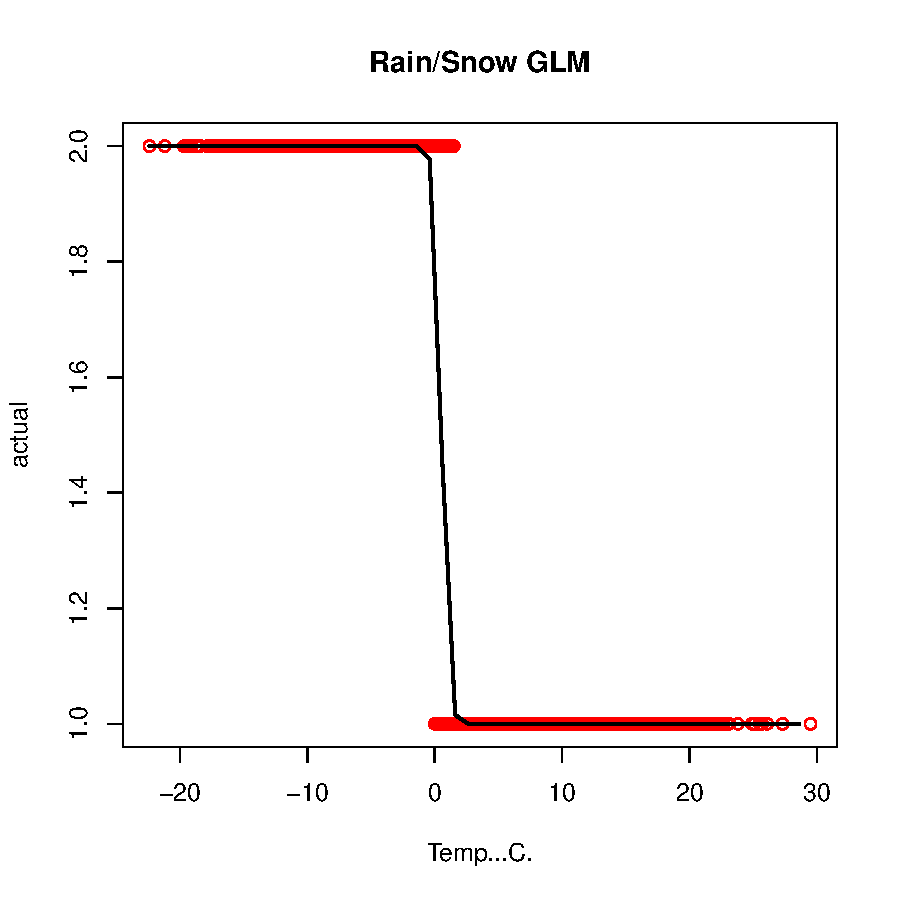
\includegraphics{datacleaning-chunk4glm}






\pagebreak

Loading in crash data:

\begin{Schunk}
\begin{Sinput}
> fullCrash = subset(read.csv('../../crashdata/Southern Interior_Full Data_data.csv'), 
+           select = - c(`Crash.Breakdown.2`, `Region`,
+                        `Municipality.Name..ifnull.`))
> summary(fullCrash)
\end{Sinput}
\begin{Soutput}
 Date.Of.Loss.Year Animal.Flag              Crash.Severity  Cyclist.Flag
 Min.   :2017      No :54118   CASUALTY CRASH      :11473   No :55725   
 1st Qu.:2018      Yes: 2018   PROPERTY DAMAGE ONLY:44663   Yes:  411   
 Median :2019                                                           
 Mean   :2019                                                           
 3rd Qu.:2020                                                           
 Max.   :2021                                                           
                                                                        
    Day.Of.Week                Derived.Crash.Configuration Heavy.Veh.Flag
 FRIDAY   :9316   REAR END                   :13024        No :54085     
 MONDAY   :8024   SINGLE VEHICLE             :12495        Yes: 2051     
 SATURDAY :6753   UNDETERMINED               :11453                      
 SUNDAY   :5464   SIDE IMPACT                :11369                      
 THURSDAY :9061   CONFLICTED                 : 3068                      
 TUESDAY  :8728   SIDE SWIPE - SAME DIRECTION: 1833                      
 WEDNESDAY:8790   (Other)                    : 2894                      
 Intersection.Crash  Month.Of.Year   Motorcycle.Flag Parked.Vehicle.Flag
 No :31677          JULY    : 5152   No :55673       No :38567          
 Yes:24459          DECEMBER: 5095   Yes:  463       Yes:17569          
                    JANUARY : 5063                                      
                    AUGUST  : 4907                                      
                    OCTOBER : 4836                                      
                    JUNE    : 4735                                      
                    (Other) :26348                                      
 Parking.Lot.Flag Pedestrian.Flag  Street.Full.Name..ifnull.
 No :37189        No :55790       HWY 97        : 6019      
 Yes:18947        Yes:  346       HARVEY AVE    : 3168      
                                  HWY 33        : 2064      
                                  GORDON DR     : 1921      
                                  LAKESHORE RD  : 1372      
                                  SPRINGFIELD RD: 1326      
                                  (Other)       :40266      
     Time.Category      Municipality.Name Road.Location.Description
 12:00-14:59:14870   KELOWNA     :45943   UNKNOWN     : 2211       
 15:00-17:59:14473   WEST KELOWNA:10193   HWY 97      : 1961       
 09:00-11:59:11021                        HARVEY AVE  : 1670       
 18:00-20:59: 5805                        LAKESHORE RD:  932       
 06:00-08:59: 5489                        LOUIE DR    :  751       
 21:00-23:59: 2684                        HWY 33      :  715       
 (Other)    : 1794                        (Other)     :47896       
       Street.Full.Name Metric.Selector Total.Crashes   Total.Victims   
 HWY 97        : 6019   Min.   :1.000   Min.   :1.000   Min.   :0.0000  
 HARVEY AVE    : 3168   1st Qu.:1.000   1st Qu.:1.000   1st Qu.:0.0000  
 HWY 33        : 2064   Median :1.000   Median :1.000   Median :0.0000  
 GORDON DR     : 1921   Mean   :1.006   Mean   :1.006   Mean   :0.2917  
 LAKESHORE RD  : 1372   3rd Qu.:1.000   3rd Qu.:1.000   3rd Qu.:0.0000  
 SPRINGFIELD RD: 1326   Max.   :3.000   Max.   :3.000   Max.   :9.0000  
 (Other)       :40266                                                   
\end{Soutput}
\end{Schunk}




\begin{Schunk}
\begin{Sinput}
> #save(alldata, file = "../rda_files/all_data.rda")
\end{Sinput}
\end{Schunk}


\end{document}
